% The Not So Short Introduction to LaTeX
%
% Copyright (C) 1995--2022 Tobias Oetiker, Marcin Serwin, Hubert Partl,
% Irene Hyna, Elisabeth Schlegl and Contributors.
%
% This document is free software: you can redistribute it and/or modify it
% under the terms of the GNU General Public License as published by the Free
% Software Foundation, either version 3 of the License, or (at your option) any
% later version.
%
% This document is distributed in the hope that it will be useful, but WITHOUT
% ANY WARRANTY; without even the implied warranty of MERCHANTABILITY or FITNESS
% FOR A PARTICULAR PURPOSE.  See the GNU General Public License for more
% details.
%
% You should have received a copy of the GNU General Public License along with
% this document.  If not, see <https://www.gnu.org/licenses/>.

% !TEX root = ./lshort.tex
%chktex-file 36
%chktex-file 8
\chapter{Graphics in Your Document}\label{chap:graphics}

\begin{intro}
  Most documents these days contain some graphics alongside the text. While
  photos and drawings can be easily added, integrating diagrams and schematics
  seamlessly with your document might prove difficult. Fonts, colours, and lines
  must be adjusted so that they do not look out of place. Furthermore, later
  changes to your document layout may force you to redo this work. Fortunately
  it is possible to create your graphics directly in \LaTeX{}, which will
  automatically take care of adjusting the aforementioned settings and keep
  them in sync with the document itself.
\end{intro}

\section{Overview}

First, some background on how to think about graphics.
Roughly, there are three types of pictures that you may find yourself
dealing with:
\begin{description}
  \item[Photos] are pictures that contain realistic shading and lots of
    detail. These include actual photos, photo-realistic
    renders, and screenshots from video games. In photos, exact pixel colour is
    not really important, and lossy compression can be used without visual
    degradation. It is best to store photos in the JPEG format.
  \item[Drawings] are pictures with flat colours and relatively few details.
    This category includes pixel art and screenshots of program
    interfaces. Here, lossy compression would result in visible degradation, and
    would not be very efficient anyway. It is best to use a lossless compression
    format such as PNG\@. This will ensure that each picture is reproduced with
    pixel-perfect fidelity, while keeping the file sizes small.
  \item[Diagrams or Charts] are simple graphics that contain text, lines, and
    other geometric objects. Logos and schematics are prime examples of these.
    Ideally, they should be stored as drawing instructions in a vector based
    graphics in format, such as EPS, SVG or PDF\@. Vector based graphics can be
    scaled to any size without loss of quality.
\end{description}

\noindent
You have already learned about including photos and drawings, in
\autoref{sec:images}. You can use the same techniques to include
diagrams, and this is totally fine. Some programs, such as
Inkscape~\cite{inkscape}, even support ways to easily include produced graphics
in \LaTeX{} documents. However, this chapter will focus on drawing diagrams
directly in \LaTeX{}. This has many advantages, such as logical structuring,
plain text formatting, and seamless integration with the document layout.

Creating graphical output with \LaTeX{} has a long tradition. It started out
with the \ei{picture} environment, which allows you to create graphics by
cleverly placing predefined elements onto a canvas. Unfortunately, this
environment is not very robust, and so many alternatives have been developed
over the years, such as \pai*{metapost}, \pai*{asymptote} or \pai*{xypic}.
Today, the most
widely used package is \pai*{pgf} (short for \enquote{Portable Graphics
  Format}) and its user interface \TikZ{} (a recursive acronym---\enquote{\TikZ{}
  ist \textit{kein} Zeichenprogramm}---German for \enquote{\TikZ{} is
  \textit{not} a drawing program}). This chapter will introduce the basic
concepts of writing graphics in \TikZ{}. More detailed tutorials can be found
in the \pai{pgf} documentation.

While \TikZ{} is a powerful and versatile language, using it for
complicated graphics is not always easy. Many packages and libraries build
upon the \pai{pgf} foundation to simplify the creation of specialized diagrams.
These include \pai*{pgfplots}, for plotting functions and presenting data, and
\pai*{commutative-diagrams}, for creating commutative diagrams. It's usually a
good idea to search CTAN for a package which already solves your problem
before writing new \TikZ{} code from the ground up, yourself.

\section{Basic Usage}

To use \pai{pgf} and \TikZ{}, simply put the following line in the
preamble:
\begin{minted}{latex}
  \usepackage{tikz}
\end{minted}
Doing so provides the \ei{tikzpicture} environment and the \csi{tikz}
command, inside of which you can execute \TikZ{} commands. Each \TikZ{} command
is terminated with a semicolon (\verb|;|). The simplest command is the
\csi{draw} command, which draws points connected by a path. Points may be given
in either Cartesian coordinates \((x, y)\) or polar coordinates
\((\theta\mathpunct{:} r)\), where \(\theta\) is specified in degrees, while
distances are specified in centimetres by default. The path
between points may be specified in many ways, the simplest is
\ltx|--|, which draws a straight line.
\begin{example}
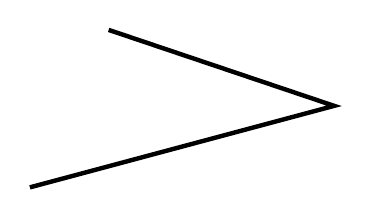
\begin{tikzpicture}
  \draw (0, 0)
    -- (15:4)
    -- (1, 2);
\end{tikzpicture}
\tikz{\draw (0, 0) -- (1,1);}
\end{example}
If you want to close the shape you are drawing, use \cargv{cycle} instead of
repeating the first point. In addition to being clearer about the intention,
it also produces a better looking line connection (a properly mitred join, as they say).
\begin{example}[vertical_mode, examplewidth=0.75\linewidth]
\begin{tikzpicture}
\begin{scope}[spy using outlines={circle, magnification=15, size=1.2cm, connect spies}] %!hide
  \draw (0, 0) -- (2, 0) -- (60: 2) -- (0, 0);
  \spy on (0,0) in node [left] at (-0.1, 0.9); %!hide
\end{scope} %!hide
\end{tikzpicture}
vs.\
\begin{tikzpicture}
\begin{scope}[spy using outlines={circle, magnification=15, size=1.2cm, connect spies}] %!hide
  \draw (0, 0) -- (2, 0) -- (60: 2) -- cycle;
  \spy on (0,0) in node [left] at (-0.1, 0.9); %!hide
\end{scope} %!hide
\end{tikzpicture}
\end{example}

The \csi{draw} command is just a shortcut to the more general \csi{path} command.
The latter accepts a path in the same way, but an action
must be specified in square brackets. The \csi{draw} command simply
supplies the \cargv{draw} action. The \cargv{fill} action fills the area under
the specified path. Multiple actions may be supplied.
\begin{example}[vertical_mode, examplewidth=0.8\linewidth]
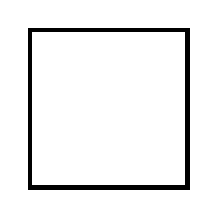
\begin{tikzpicture}
  \path[draw]
    (0, 0) -- (0, 2) -- (2, 2) -- (2, 0) -- cycle;
\end{tikzpicture}

\begin{tikzpicture}
  \path[fill]
    (0, 0) -- (0, 2) -- (2, 2) -- (2, 0) -- cycle;
\end{tikzpicture}
\end{example}

By default, \TikZ{} pictures adjust their size to the minimal surrounding
rectangle. If you want to specify the bounding box yourself, use the
\cargv{use as bounding box} action, or the equivalent \csi{useasboundingbox}
command.
\begin{chktexignore}
\begin{example}[vertical_mode, examplewidth=0.6\linewidth]
\tikz{\draw (0, 0) -- (1, 0);}
vs.\
\tikz{\draw (0, 1) -- (1, 1);}
vs.\
\tikz{
  \useasboundingbox (0, 0) -- (0, 1)
    -- (1, 1) -- (1, 0) -- cycle;
  \draw (0, 1) -- (1, 1);
}
\end{example}
\end{chktexignore}

Normal \LaTeX{} input may be displayed inside so-called nodes. To create
a node, use the
\begin{lscommand}
  \csi{node}[«{}» («\bs carg{name}») at «\bs carg{coordinate}» {«\bs carg{input}»};: c]
\end{lscommand}
command. The \carg{name} argument is optional and enables you to use the
\carg{name} as a shorthand for a node's coordinate.

\begin{example}
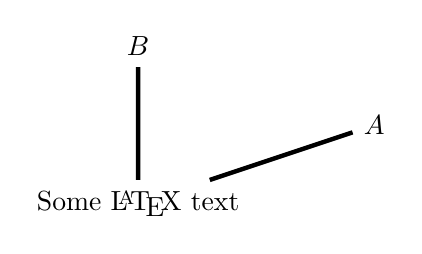
\begin{tikzpicture}
  \node (text) at (0,0) {%
    Some \LaTeX{} text};
  \node (A) at (3, 1) {\(A\)};
  \node (B) at (0, 2) {\(B\)};
  \draw (A) -- (text) -- (B);
\end{tikzpicture}
\end{example}
\TikZ{} attempts to be smart about the way it positions lines between nodes.
If you want to influence this, you can specify the exact connection-point on a node
after a dot. The available points are, for example, \cargv{north},
\cargv{west}, \cargv{south east} and so on. You can also put a number, which
will be interpreted as an angle (in degrees).
\begin{example}
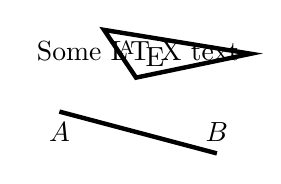
\begin{tikzpicture}
  \node (T) at (1,1) {%
    Some \LaTeX{} text};
  \node (A) at (0, 0) {\(A\)};
  \node (B) at (2, 0) {\(B\)};
  \draw (A.north) -- (B.south);
  \draw (T.0) -- (T.145)
    -- (T.265) -- cycle;
\end{tikzpicture}
\end{example}

Nodes can be created within paths by typing \ltx{node}
after a given coordinate or line. A node added after a line
is placed at its midpoint.
\begin{example}
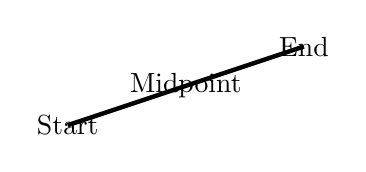
\begin{tikzpicture}
  \draw (0, 0) node {Start}
    -- node {Midpoint}
    (3, 1) node {End};
\end{tikzpicture}
\end{example}

If you want to create an empty node for the purpose of naming a specific point,
it is better to use the \csi{coordinate} command. This
ensures that the node is actually empty, whereas nodes created by \csi{node}
take up some space by default, even when they have no content.
\begin{example}
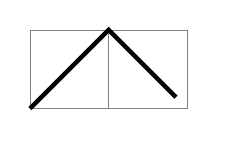
\begin{tikzpicture}
  \draw [help lines] (0, 0) grid (2, 1); % !hide
  \coordinate (A) at (0, 0);
  \coordinate (B) at (1, 1);
  \node (C) at (2, 0) {};
  \draw (A) -- (B) -- (C);
\end{tikzpicture}
\end{example}

\section{Curves and Shapes}

So far we have always used \ltx|--| to connect points. However,
this is not the only way. For example, if you wanted to only use horizontal and
vertical lines, you could specify \ltx/-|/ or \ltx/|-/ (according to preferred
order) as the connection between points.
\begin{example}
\tikz{\draw (0, 0) |- (2, 1);}
\tikz{\draw (0, 0) -| (2, 1);}
\end{example}

If you want to create curved lines, the simplest way is to use \ltx{to}
between points. It works the same as \ltx{--}, but you can provide an optional
argument, with \cargv{in} and \cargv{out} keys, to define the terminal angles of
the connection.
\begin{example}[vertical_mode, examplewidth=0.8\linewidth]
\tikzset{baseline} \vspace{-0.3cm} %!hide
\tikz{\draw (0, 0) to[out=90, in=-90] (2, 0);}
\tikz{\draw (0, 0) to[out=45] (2, 0);}
\vspace{-0.5cm} %!hide
\end{example}
The \cargv{looseness} key may be used to define how much the curve is
outstretched.
\begin{example}[vertical_mode, examplewidth=0.8\linewidth]
\tikzset{baseline} \vspace{-1cm} %!hide
\tikz{\draw (0, 0)
  to[out=90, in=-90, looseness=0.5] (2, 0);}
\tikz{\draw (0, 0)
  to[out=90, in=-90, looseness=2] (2, 0);}
\vspace{-1cm} %!hide
\end{example}
Often it might be easier to specify relative angles, using the \cargv{bend
  left} and \cargv{bend right} keys. If no angle is provided, a default value is
used.
\begin{example}[vertical_mode, examplewidth=0.8\linewidth]
\tikz{\draw (0, 0) to[bend left] (2, 0);}
\tikz{\draw (0, 0) to[bend right=90] (2, 0);}
\end{example}

If you need even finer control over the curves you, can use a
\ltx{.. controls ..} connection to specify a Bézier curve with one
or two control points.
\begin{chktexignore}
\begin{example}[vertical_mode, examplewidth=0.8\linewidth]
\vspace{-0.5cm} %!hide
\tikz{\draw (0, 0) .. controls (1, 1) .. (2, 0);}
\tikz{\draw (0, 0) .. controls (.5, 2) and (3, 1)
  .. (2, 0);}
\end{example}
\end{chktexignore}

In addition to curves, the points may also be connected using various shapes.
For example, the \ltx{grid} draws a grid between the points, while
\ltx{rectangle} draws a rectangle.
\begin{example}[vertical_mode, examplewidth=0.8\linewidth]
\tikz{\draw (0, 0) grid (2, 2);}
\tikz{\draw (0, 0) rectangle (3, 1);}
\end{example}
To specify how fine the grid is, use the \cargv{step} key.
\begin{example}[vertical_mode, examplewidth=0.8\linewidth]
\tikz{\draw (0, 0) grid[step=0.5] (2, 2);}
\tikz{\draw (0, 0) grid[step=1.5] (2, 2);}
\end{example}

Other shapes may also be drawn this way, sometimes requiring a specific syntax.
For example the \ltx{circle} interprets the left coordinate as its centre and
receives its radius via the \cargv{radius} key. You can also specify \cargv{x
  radius} and \cargv{y radius} separately, thus drawing an ellipse.\footnote{The
  \cargv{ellipse} shape can also be used in the same way if the naming irks you
  \smiley.}
\begin{example}[vertical_mode, examplewidth=0.9\linewidth]
\tikz{\draw (0, 0) circle[radius=1];}
\tikz{\draw (0, 0) circle[x radius=2, y radius=0.5];}
\end{example}
Many more shapes are available, such as \ltx{arc}, \ltx{parabola} or \ltx{sin}.
Be sure to check out the documentation\cite{pack:pgf} for the specifics of their use.

\section{Customizing Paths and Nodes}

By default, all paths are drawn with a continuous black line. You can modify
them by passing options to the \csi{draw} command. For example, passing
a colour name will change the colour of the line.
\begin{example}
\tikz{\draw[red]
  (0, 0) -- (1, 1);}
\tikz{\draw[blue]
  (0, 0) -- (1, 1);}
\end{example}

The thickness of a line can be controlled by passing the \cargv{line width} key
(specified in points by default), or by using one of the predefined values, such
as \cargv{semithick}, \cargv{very thin} or \cargv{ultra thick}.
\begin{example}
\tikz{\draw[line width=2]
  (0, 0) -- (1, 1);}
\tikz{\draw[very thin]
  (0, 0) -- (1, 1);}
\end{example}

The endings of lines can also be customized. For
example, \cargv{line cap} allows you to specify rounded
end-caps.
\begin{example}
\tikz{\draw[line width=10]
  (0, 0) -- (1, 1);}
\tikz{\draw[line width=10,
  line cap=round]
  (0, 0) -- (1, 1);}
\end{example}
You can turn a line into an arrow by specifying the \cargv{arrows} key.
\begin{example}
\tikz{\draw[arrows=->]
  (0, 0) -- (1, 1);}
\tikz{\draw[arrows=<<->]
  (0, 0) -- (1, 1);}
\end{example}

Lines do not need to be continuous, either. You can specify a \cargv{dash
  pattern} or use one of the predefined patterns.
\begin{example}
\tikz{\draw[dash pattern=
  on 4 off 1 on 2 off 1]
  (0, 0) -- (1, 1);}
\tikz{\draw[dotted]
  (0, 0) -- (1, 1);}
\end{example}

Adjust how lines are connected by using
\cargv{line join}. Set it to \cargv{round}, \cargv{bevel}, or
\cargv{miter}.
\begin{example}
\tikzset{every picture/.style={line width=6pt}} %!hide
\tikz{\draw[line join=round]
  (0, 0) -- (0.5, 1) -- (1, 0);}
\tikz{\draw[line join=bevel]
  (0, 0) -- (0.5, 1) -- (1, 0);}
\end{example}
If you want the line joins to be rounded, you can also pass the \cargv{rounded
  corners} key with the value set to the radius of the arc.
\begin{example}
\tikz{\draw[rounded corners]
  (0, 0) -- (0.5, 1) -- (1, 0);}
\tikz{\draw[rounded corners=25]
  (0, 0) -- (0.5, 1) -- (1, 0);}
\end{example}

Now, let's turn our attention to nodes. By default, a node's boundary is not
drawn, but you can pass \cargv{draw} and \cargv{fill}, optionally set to a
colour, to reveal it.
\begin{example}
\tikz{\node[draw] (0, 0)
  {Some Text};}
\tikz{\node[fill=red] (0, 0)
  {Some Text};}
\end{example}
By default, all nodes are rectangles, but they can be changed to circles by
passing the \cargv{circle} key to their options.
\begin{example}
\tikz{\node[draw, circle]
  (0, 0) {Some text};}
\end{example}

If you want to place multi-line text inside a node, you have to specify the
\cargv{align} key; without it, new lines are ignored. Possible values
are \cargv{left}, \cargv{center} and \cargv{right}.
\begin{example}
\tikz{\node[draw, align=left]
  (0, 0) {Some more\\ text};}
\tikz{\node[draw, align=center]
  (0, 0) {Even more \\ text};}
\end{example}

When nodes are placed along a path, their positions may be adjusted using the
\cargv{anchor} key. Its value is the point on the node boundary that should be
anchored on the given point in path.
\begin{example}
\tikz{\draw
  (0, 0) node[anchor=south] {A}
  -- node[anchor=north west] {B}
  (1, 1) node[anchor=135] {C};
}
\end{example}
Using relative commands, such as \cargv{left} or \cargv{above right}, for this
purpose usually leads to more readable code, though they are not so powerful.
\begin{example}
\tikz{\draw
  (0, 0) node[above] {A}
  -- node[below right] {B}
  (1, 1) node[right] {C};
}
\end{example}

All these options can be freely combined, but the resulting style specification
may turn out to be lengthy. To avoid retyping it for many nodes or paths, you
can define new styles. Some predefined styles already exist. For example, the
\cargv{help lines} style sets the colour of the lines to grey and makes them a bit
thinner, which is useful for drawing alignment grids when constructing your own
pictures.
\begin{example}
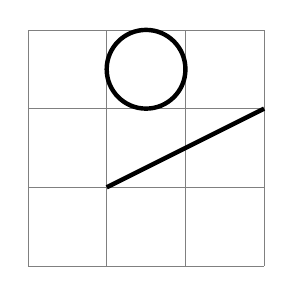
\begin{tikzpicture}
  \draw[help lines]
    (0, 0) grid (3,3);
  \draw (1, 1) -- (3,2);
  \draw (1.5, 2.5)
    circle[radius=0.5];
\end{tikzpicture}
\end{example}
To define your own style, pass a key of the form
\cargv{\carg{name}/.style=\carg{options}} to the \TikZ{} environment or
command options.
\begin{example}[vertical_mode, examplewidth=0.7\linewidth]
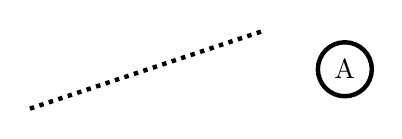
\begin{tikzpicture}[
  my line/.style={dotted, ultra thick},
  my node/.style={draw, circle},
]
  \draw[my line] (0, 0) -- (3, 1);
  \node[my node] at (4, 0.5) {A};
\end{tikzpicture}
\end{example}
If you want to set up some styles globally, you can also use the \csi{tikzset}
command.
\begin{example}
\tikzset{
  red style/.style={draw=red},
}
\tikz{\draw[red style]
  (0, 0) -- (1, 1) -- (2, 0);}
\tikz{\node[red style]
  at (0, 0) {Red node};}
\end{example}
If you want to avoid specifying the style for every node or path within a
\TikZ{} picture, you can set the special styles \cargv{every node} and
\cargv{every path} to change them all at once.
\begin{example}
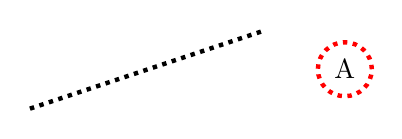
\begin{tikzpicture}[
  every path/.style={
    ultra thick, dotted},
  every node/.style={
    circle, draw=red},
]
  \draw (0, 0) -- (3, 1);
  \node at (4, 0.5) {A};
\end{tikzpicture}
\end{example}

\section{Coordinates}

So far, we have always used the default unit of centimetres for specifying
coordinates. However, it is possible to use any \LaTeX{} dimension (see
\autoref{sec:dimensions} for details).
\begin{example}
\tikz{\draw (0, 0)
  -- (1in, 1pt);}
\tikz{\draw (0, 0)
  -- (1dd, 1em);}
\end{example}

It is also possible to rescale how the distances are measured by using the
\cargv{scale} key. This is useful if you find that your picture is too big or
too small after drawing it, or if there exists some intuitive coordinate system
(for example, when drawing function plots).
\begin{example}
\tikz[scale=2]{\draw
  (0, 0) -- (1, 1);}
\tikz{\draw (0, 0) -- (2, 2);}
\end{example}
You can also specify \cargv{xscale} and \cargv{yscale} separately.

When specifying scale, you can use simple arithmetic operations. For example, to
change the dimensionless values to inches, you can pass \ltx{scale=1in/1cm}.
\begin{example}
\tikz[scale=1in/1cm]{\draw
  (0, 0) -- (1, 0.5);}
\tikz[scale=1em/1cm]{\draw
  (0, 0) -- (1, 0.5);}
\end{example}
Keep in mind that coordinates with dimensions will also be scaled, which may
have unintended consequences. A more robust way of changing dimensionless
values is the \cargv{x} and \cargv{y} keys.
\begin{example}
\tikz[x=1in, y=1in]{\draw
  (0, 0) -- (1, 0.5);}
\tikz[x=1em, y=10ex]{\draw
  (0, 0) -- (1, 0.5);}
\end{example}

You can actually specify three-dimensional coordinates when drawing pictures.
By default, the third coordinate is interpreted as a vector pointing \(45\)
degrees to the bottom left and is a bit shorter.\footnote{Formally,
  \((0, 0, 1)\) is  the same as \((-0.385, -0.385)\).}
This gives the effect of a parallel (or axonometric) projection.
\begin{example}[vertical_mode, examplewidth=0.85\linewidth]
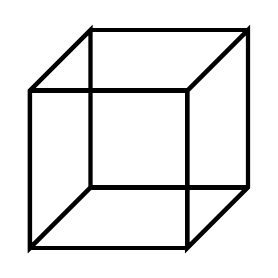
\begin{tikzpicture}[scale=2]
  \draw (0, 0, 0) -- (0, 0, 1) -- (0, 1, 1) --
    (0, 1, 0) -- cycle;
  \draw (1, 0, 0) -- (1, 0, 1) -- (1, 1, 1) --
    (1, 1, 0) -- cycle;
  \draw (0, 0, 0) -- (1, 0, 0) (0, 0, 1) -- (1, 0, 1)
    (0, 1, 1) -- (1, 1, 1) (1, 1, 0) -- (0, 1, 0);
\end{tikzpicture}
\end{example}
Length and direction can be changed by using the \cargv{z} key.

Sometimes, it may be easier to specify a path by using coordinates relative to
the previous point instead of absolute ones. To do so, prepend \ltx{++} to the
coordinate, which will be interpreted as the previous specified point plus
this vector.
\begin{example}
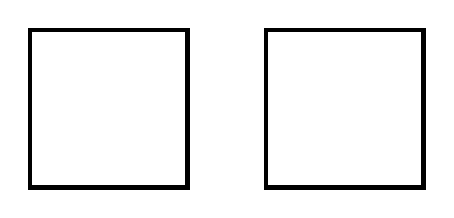
\begin{tikzpicture}[scale=2]
  \draw (0, 0) -- ++(0, 1) --
    ++(1, 0) -- ++(0, -1) --
    cycle;
  \draw (1.5, 0) -- ++(0, 1) --
    ++(1, 0) -- ++(0, -1) --
    cycle;
\end{tikzpicture}
\end{example}

Scaling is not the only transformation that can be applied to points. It is
also possible to rotate, shift, or apply an arbitrary linear transformation by
specifying its matrix. Check out the documentation for a detailed description.
\begin{example}
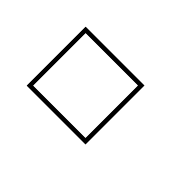
\begin{tikzpicture}[rotate=45]
  \draw (0, 0) -- (0, 1) --
    (1, 1) -- (1, 0) -- cycle;
\end{tikzpicture}
\end{example}
It is also possible to apply transformations to a single command.
\begin{example}
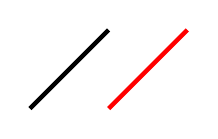
\begin{tikzpicture}
  \draw (0, 0) -- (1, 1);
  \draw[red, xshift=1cm]
    (0, 0) -- (1, 1);
\end{tikzpicture}
\end{example}
If you want to apply the same transformation to more than one command within
the same picture, you can use the \ei{scope} environment. It is especially useful
when your picture consists of more than one sub-picture, each of which is more
or less independent.
\begin{example}[vertical_mode, examplewidth=0.7\linewidth]
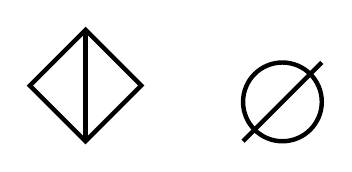
\begin{tikzpicture}
  \begin{scope}[rotate=45]
    \draw (0, 0) rectangle (1, 1);
    \draw (0, 0) -- (1, 1);
  \end{scope}
  \begin{scope}[xshift=2cm]
    \draw (0.5, 0.5) circle [radius=0.5];
    \draw (0, 0) -- (1, 1);
  \end{scope}
\end{tikzpicture}
\end{example}

When \TikZ{} pictures are positioned within text, their bottom end sits on the
baseline of the text. If you want to modify this, you can use the \cargv{baseline} key
to set the \(y\) coordinate at which the baseline should be. If no position is
specified, it defaults to \(0\).
\begin{example}[vertical_mode, examplewidth=0.8\linewidth]
text \tikz{\draw (0, 0) circle [radius=1em];}
text \tikz[baseline]{\draw
  (0, 0) circle [radius=1em];}
text \tikz[baseline=-0.5ex]{\draw
  (0, 0) circle [radius=1em];} text
\end{example}

\section{Reusing Pictures}

Sometimes, you may wish to draw the same picture at a few places within a bigger
one. While you could use the commands described in
\autoref{sec:simple_commands}, this would be problematic, since modifying their
placement or style is non-trivial. \TikZ{} comes with its own method of
defining smaller pictures, called `pics'. They can be created by passing
\cargv{\carg{name}/.pic=\carg{commands}} to the \TikZ{} environment or command,
and are then used by invoking the \csi{pic} command. An example is
presented in \autoref{lst:pics}.
\begin{listing}
  \begin{example}[vertical_mode, examplewidth=0.9\linewidth]
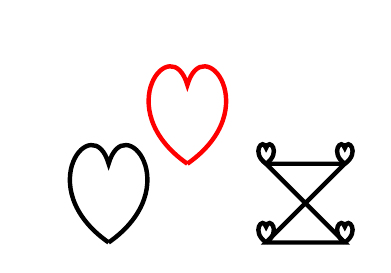
\begin{tikzpicture}[
  heart/.pic={
    \draw (0,0) .. controls (-1, 0.7) and (-0.2, 1.7)
    .. (0, 1) .. controls  (0.2, 1.7) and (1, 0.7)
    .. (0, 0);
  },
]
  \pic at (0, 0) {heart};
  \pic[red] at (1, 1) {heart};

  \begin{scope}[xshift=2cm, every pic/.style={scale=0.2}]
    \draw (0, 0) pic {heart} -- (1, 1) pic {heart} --
      (0, 1) pic {heart} -- (1, 0) pic {heart} -- cycle;
  \end{scope}
\end{tikzpicture}
\end{example}
  \caption{An example of using pics in \TikZ{}.}\label{lst:pics}
\end{listing}

If you find yourself repeating a lot of simple commands (for example, drawing
ticks on an axis), you may simplify your code by using the \csi{foreach} command. It
repeats the drawing command for each value in a list, so that you can
write repeatable code once, and need only modify the important parts.
\begin{example}[vertical_mode, examplewidth=0.8\linewidth]
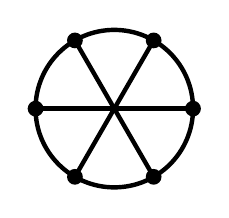
\begin{tikzpicture}
  \draw (0, 0) circle[radius=1cm];
  \foreach \i in {0, 60, 120, 180, 240, 300} {
    \draw (0, 0) -- (\i: 1);
    \fill (\i: 1) circle[radius=0.1cm];
  }
\end{tikzpicture}
\end{example}
If your values are a simple arithmetic sequence, you need only provide the first
two values and the last, replacing the rest with triple dots.
\begin{example}[vertical_mode, examplewidth=0.8\linewidth]
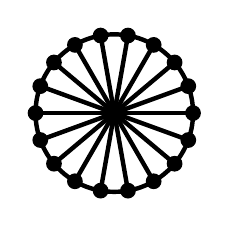
\begin{tikzpicture}
  \draw (0, 0) circle[radius=1cm];
  \foreach \i in {0, 20, ..., 340} {
    \draw (0, 0) -- (\i: 1);
    \fill (\i: 1) circle[radius=0.1cm];
  }
\end{tikzpicture}
\end{example}
You can also iterate over pairs by separating respective parts with \ltx{/}.
\begin{example}
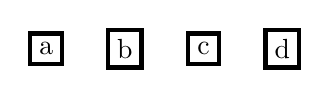
\begin{tikzpicture}
  \foreach \i/\j in {0/a,
    1/b, 2/c, 3/d} {
    \node[draw] at (\i, 0) {\j};
  }
\end{tikzpicture}
\end{example}

\section{Libraries}

\pai{pgf} and \TikZ{} do not rely on \LaTeX{}. In fact, they can be used with
any \TeX{} based system or even \TeX{} itself. For this reason, \TikZ{}
provides its own system of extensions that does not use \LaTeX{}'s
\cs{usepackage} command. Extensions of \TikZ{} are called libraries, and can be
loaded using the \csi{usetikzlibrary} command, which receives a list of comma
separated libraries.

For example, if you intend to draw some geometry problems, you will often find
yourself looking for intersections of objects. While you could calculate
their exact coordinates by hand, the \cargv{intersections} library will do it
for you. An example is presented in \autoref{lst:intersections}.

\begin{listing}
  \begin{example}[vertical_mode, examplewidth=0.8\linewidth]
%!showbegin !hide
% In preamble
\usetikzlibrary{intersections}
% ...
%!showend !hide

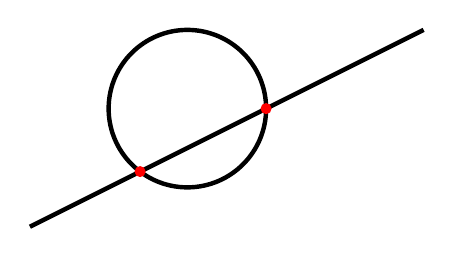
\begin{tikzpicture}
  \draw[name path=O] (0, 0) circle [radius=1];
  \draw[name path=L] (-2, -1.5) -- (3, 1);

  \fill[red, name intersections={of=O and L}]
    (intersection-1) circle[radius=2pt]
    (intersection-2) circle[radius=2pt];
\end{tikzpicture}
\end{example}
  \caption{An example of using \cargv{intersections}
    library.}\label{lst:intersections}
\end{listing}

Other libraries extend the number of available shapes. For example, the
\cargv{arrows.meta} library defines numerous additional arrow tips, if you do
not like the classical one. Some are presented in
\autoref{lst:arrows.meta}.

\begin{listing}
  \begin{example}[vertical_mode, examplewidth=0.8\linewidth]
%!showbegin !hide
% In preamble
\usetikzlibrary{arrows.meta}
% ...
%!showend !hide

\tikzset{every path/.style={ultra thick}} %!hide2
\tikz{\draw[->] (0, 0) -- (1, 1);}
\tikz{\draw[-{Circle}] (0, 0) -- (1, 1);}
\tikz{\draw[-{Stealth}] (0, 0) -- (1, 1);}
\tikz{\draw[-{Stealth[round]}] (0, 0) -- (1, 1);}
\tikz{\draw[-{Diamond[open]}] (0, 0) -- (1, 1);}
\end{example}
  \caption{Some of the arrow tips defined by \cargv{arrows.meta}
    library.}\label{lst:arrows.meta}
\end{listing}

You can perform additional calculations on existing
coordinates. The \cargv{calc} library allows you to do so by enclosing them
within \verb|$| symbols. An example is presented in
\autoref{lst:calc}.

\begin{listing}
  \begin{example}[vertical_mode, examplewidth=0.8\linewidth]
%!showbegin !hide
% In preamble
\usetikzlibrary{calc}
% ...
%!showend !hide

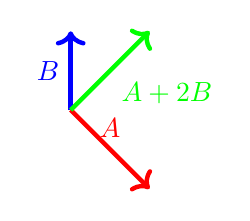
\begin{tikzpicture}
  \coordinate (A) at (1, -1);
  \coordinate (B) at (0, 1);
  \draw[red, ->] (0, 0) -- node[above] {\(A\)} (A);
  \draw[blue, ->] (0, 0) -- node[left] {\(B\)} (B);
  \draw[green, ->] (0, 0) --
      node[below right] {\(A+2B\)} ($(A)+2*(B)$);
\end{tikzpicture}
\end{example}
  \caption{An example of using the \cargv{calc} library.}\label{lst:calc}
\end{listing}

If you have a lot of \TikZ{} code in your document, you may notice that
compiling it takes much longer. This is because
\TikZ{} redraws each picture with every \LaTeX{} pass. If this becomes
annoying, you can cache your images to external files and reuse them on
subsequent runs. To do this, simply put the following code in your preamble.
\begin{minted}{latex}
\usetikzlibrary{external}
\tikzexternalize
\end{minted}
This method has some limitations, but should be sufficient for most uses. Read
up on it in the documentation if problems occur.

These are not the only libraries---additional node shapes, real 3D-perspective,
matrices, mind maps and many more are covered. Most of them are described in
the \pai*{pgf} package documentation. Check it out if you haven't found
solution to your problem here.

